
\chapter{计算机程序的物理模型及并行架构}
\label{chap:Algorithm}

\section{物理模型简介}
加速器是加速带电粒子束流的机器。我们面临的主要问题也是在束流中,其中空间电荷效应是其中非常重要的一种。
针对空间电荷问题,我们主要有两种描述手段,分别是使用解析的方法和数值的方法,其中解析的方法为求解傅拉梭夫方程(Vlasov Equation),如式\ref{eq:Vlasov}。
\begin{equation}
    \label{eq:Vlasov}
    \begin{aligned}
        & f(x,y,z,{{p}_{x}},{{p}_{y}},{{p}_{z}})=f(H) \\
        & \frac{df}{dt}=0 \\
        & \Delta U=-\frac{\rho }{{{\varepsilon }_{0}}} \\
    \end{aligned}
\end{equation}

但是多体耦合问题是没有解析解的,我们必须采用一些近似,建立一个更简单的模型,以得到这个问题的大致图像。
T. P. Wangler在1998年提出了了一种束核模型\cite{wangler1998particle}以描述空间电荷导致的束晕形成机制。
在束核模型中,连续的束流通过一个轴对称的聚焦通道,假设粒子束核为均匀分布,则其包络大小可由包络方程描述。此时一个任意的粒子会受到束核产生的空间电荷力,当粒子处于束核内部时,空间电荷力为线性的;当粒子处于束核外部时,空间电荷力为非线性的。
忽略单粒子对束核的影响,则束核的半径可以由式\ref{eq:particle_core_envelope}表示。
\begin{equation}
    \label{eq:particle_core_envelope}
    \frac{{{d}^{2}}R}{d{{z}^{2}}}+k_{0}^{2}R-\frac{{{\varepsilon }^{2}}}{{{R}^{3}}}-\frac{K}{R}=0
\end{equation}

其中
\begin{equation}
K=\frac{qI}{2\pi \varepsilon m{{c}^{3}}{{\beta }^{3}}{{\gamma }^{3}}}
\end{equation}

式中$R$为束核包络的大小,$q$,$m$,和$\beta c$分别为粒子的电荷,质量,和纵向速度,$k_{0}$为外部聚焦强度,$\gamma$为洛伦兹因子,$I$为流强,$\varepsilon$为发射度。

而单粒子的横向运动方程如式\ref{eq:particle_core_singleparticle}:
\begin{equation}
    \label{eq:particle_core_singleparticle}
    \frac{{{\text{d}}^{2}}X}{\text{d}{{z}^{2}}}+k_{0}^{2}X-{{F}_{sc}}=0
\end{equation}

其中$X$为粒子的横向位置,${F}_{sc}$为由均匀分布束核产生的的空间电荷力,可以表示为:
\begin{equation}
{{F}_{sc}}=\left\{
        \begin{aligned}
        & KX/{{R}^{2}}, &\left| X \right|<R \\
        & K/X,          &\left| X \right|\ge R \\
        \end{aligned} \right.
\end{equation}

对式\ref{eq:particle_core_envelope}和式\ref{eq:particle_core_singleparticle}进行无量纲化,我们引入以下变量$r=R/R_0$,$x=X/R_0$,$\tau = k_0 z $,并将空间电荷导致的相位压缩因子表示为$\eta = k/k_0 = \sqrt{1+u^2}-u$。则无量纲化的束核包络方程可以表示为:
\begin{equation}
    \label{eq:particle_core_envelope_dimensionless}
    \frac{{{d}^{2}}r}{d{{\tau}^{2}}}+r-\frac{{{\eta }^{2}}}{{{r}^{3}}}-\frac{1-{\eta}^2}{r}=0
\end{equation}
无量纲化的单粒子运动方程可以表示为:
\begin{equation}
    \label{eq:particle_core_singleparticle_dimensionless}
    \frac{{{d}^{2}}x}{d{{\tau}^{2}}}+x-(1-{\eta}^2) \times \left\{
        \begin{aligned}
        & x/{{r}^{2}}, &\left| x \right|<r \\
        & 1/x,         &\left| x \right|\ge r \\
        \end{aligned} \right.
\end{equation}

对式\ref{eq:particle_core_envelope_dimensionless}和式\ref{eq:particle_core_singleparticle_dimensionless}
仅含有相位压缩因子$\eta$一个参数。束核的匹配解为$r=1$,为了描述束核的初始匹配程度,我们将束核的初始的包络半径定位为失配度$\mu = r_{initial}$。

失配度会影响束核包络的变化。当束核完全与聚焦强度完全匹配时,即$\mu = 1$时,束核的包络大小是不变的;而当包络与聚焦强度不匹配的时候,包络半径会周期性变化,如图\ref{fig:particle_core_envelope}的蓝色曲线为$\eta = 0.5$,$\mu = 0.6$时的束核半径变化情况。
而粒子和束核的相互作用会驱使粒子横向位置发生变化,以表示空间电荷对粒子的影响,如图\ref{fig:particle_core_envelope}的红色曲线为粒子初始$x=0.8$,$x'=0$时的粒子横向轨迹。

\begin{figure}[!tbh]
    \centering
    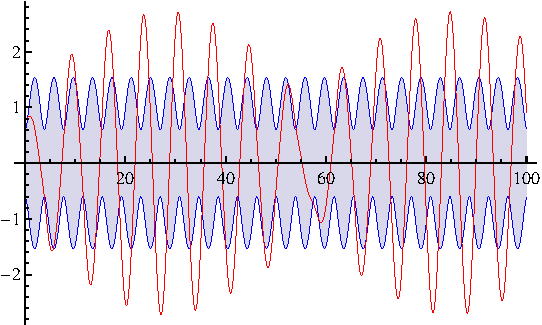
\includegraphics[width=0.65\textwidth]{Img/particle_core_envelope.pdf}
    \caption{束核包络与单粒子横向位移}
    \label{fig:particle_core_envelope}
\end{figure}

可以看出,束核的半径呈现规律的周期震荡。而当在每个周期的开始处对粒子的横向位置和动量进行观测时,我们可以得到一张粒子的庞加莱截面(Poincare surface of section),如图\ref{fig:particle_core_particle}所示,在粒子的庞加莱截面中可以看到明显的规律,粒子沿着某一条轨道进行运动。
\begin{figure}[!tbh]
    \centering
    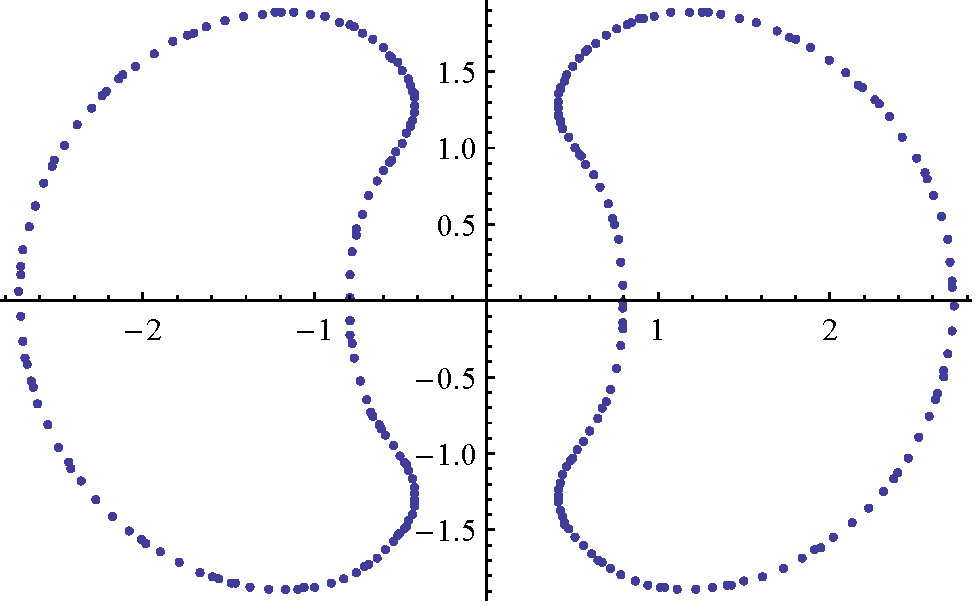
\includegraphics[width=0.65\textwidth]{Img/particle_core_particle.pdf}
    \caption{粒子的庞加莱截面}
    \label{fig:particle_core_particle}
\end{figure}

对粒子从中心到边界均匀排布,我们可以得到一组庞加莱截面,以显示不同初始位置处粒子的行为,如图\ref{fig:particle_core_Poincare}所示。四副图分别为不同的相位压缩因子$\eta$下的庞加莱截面,不同的颜色代表不同初始位置的粒子的轨迹。
\begin{figure}[!htbp]
  \centering
  ~%add desired spacing
  \begin{subfigure}[b]{0.6\textwidth}
    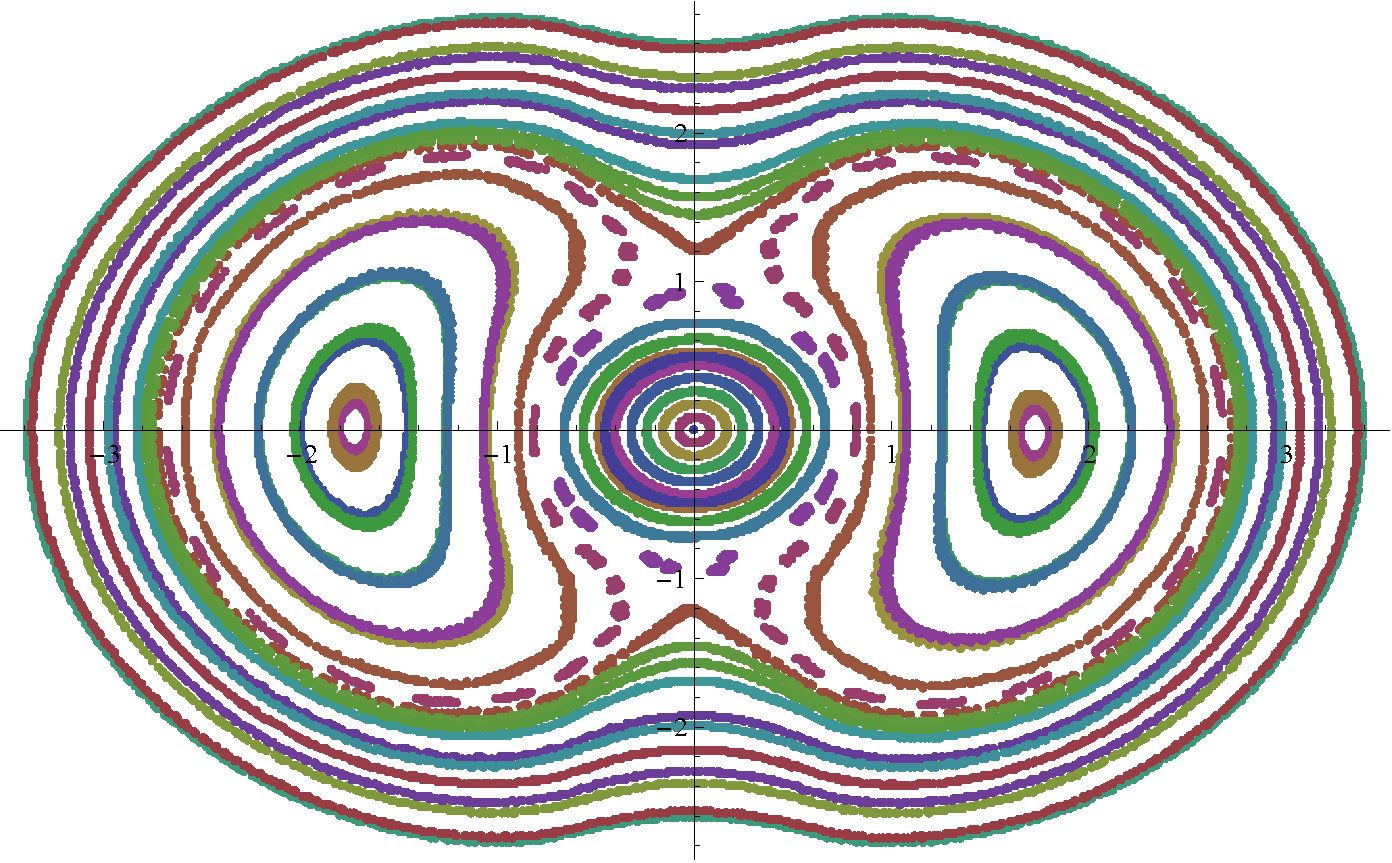
\includegraphics[width=\textwidth]{particle_core_Poincare5.pdf}
    \caption{$\eta = 0.5$}
    \label{fig:particle_core_Poincare5}
  \end{subfigure}
  ~
  \begin{subfigure}[b]{0.6\textwidth}
    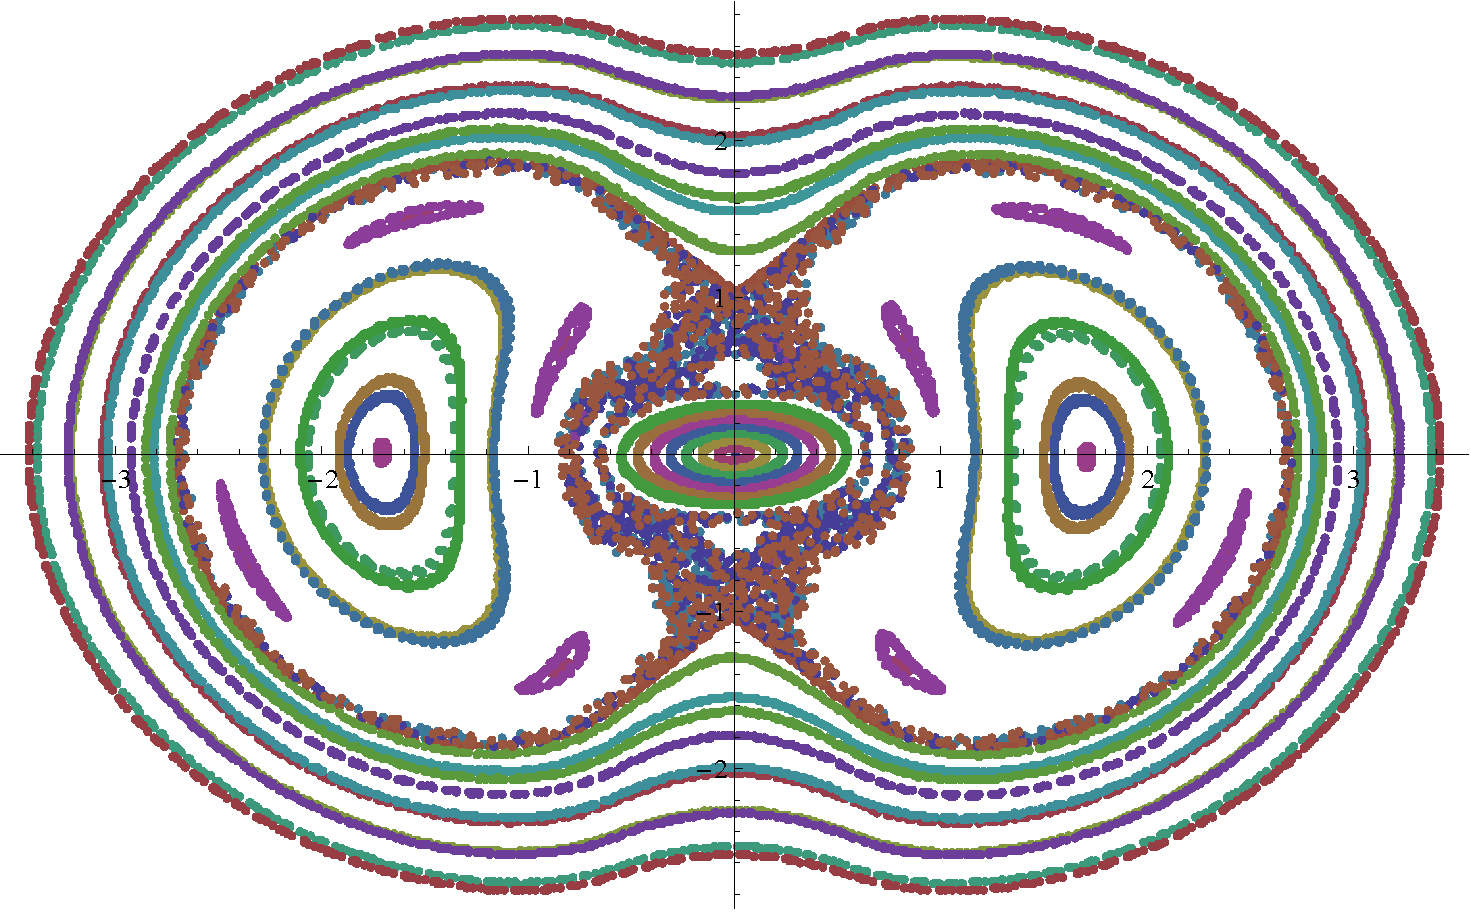
\includegraphics[width=\textwidth]{particle_core_Poincare3.pdf}
    \caption{$\eta = 0.3$}
    \label{fig:particle_core_Poincare3}
  \end{subfigure}%
  ~
  \begin{subfigure}[b]{0.6\textwidth}
    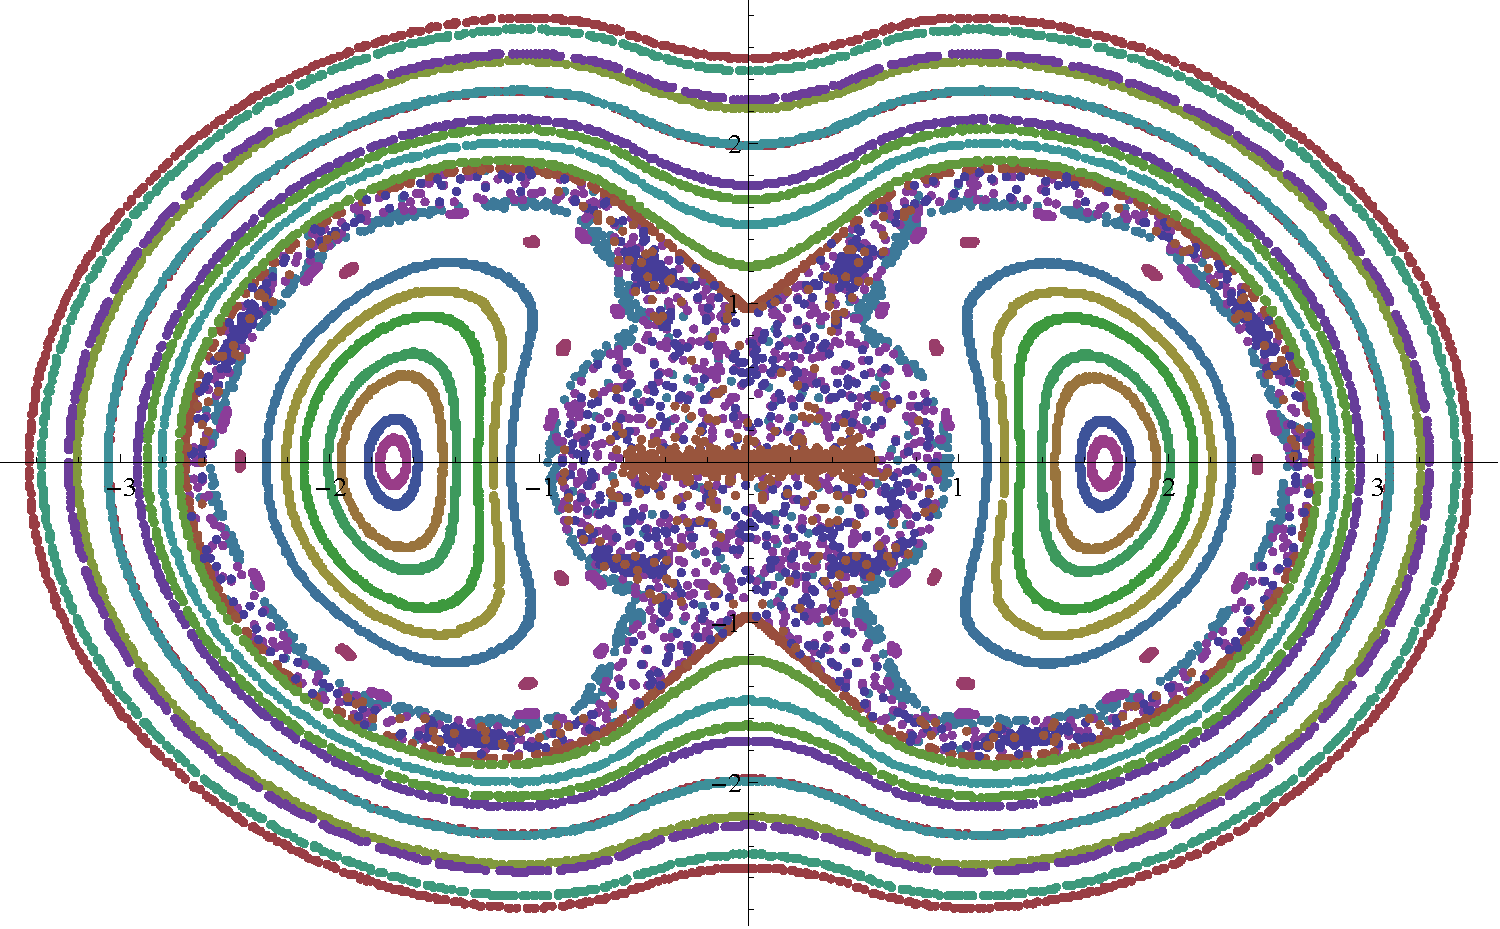
\includegraphics[width=\textwidth]{particle_core_Poincare1.pdf}
    \caption{$\eta = 0.1$}
    \label{fig:particle_core_Poincare1}
  \end{subfigure}%
  \caption{不同相位压缩因子下的庞加莱截面}
  \label{fig:particle_core_Poincare}
\end{figure}

庞加莱截面图可以分为三个区域:一,内椭圆区,大小约为束核半径及周边一小部分;二,不动点区,或者叫共振区,包括x轴上的不动点以及周围的环线,显示了参数共振的轨迹;三,外围类椭圆轨迹。
在空间电荷效应较弱的情况下,即$\eta$较大时,三个区的粒子都是做有规律的运动如图\ref{fig:particle_core_Poincare5}所示。但是当空间电荷主导的时候,比如$\eta=0.1$和$\eta=0.3$的时候(图\ref{fig:particle_core_Poincare3}和图\ref{fig:particle_core_Poincare1}),在内椭圆区会出现混沌行为,并且随着相位压缩因子变小,混沌行为变得更加明显,参数区的粒子轨迹也开始对初始条件敏感。

由庞加莱截面可以对束晕形成的机制进行分析,束晕中的粒子主要来源于共振区中的粒子,这些粒子最开始分布于内椭圆区与共振区的分界线附近,随着粒子运动,其向外移动到共振区与外椭园区的边界附近,在两个边界间震荡,形成了束晕。在空间电荷效应主导的情况下,内椭圆区的粒子也有可能形成束晕,如图\ref{fig:particle_core_Poincare1}所示,内椭圆区也出现了了混沌行为,最内部的粒子也会移动到外部形成束晕。

束核模型在一定程度上可以解释束晕形成的机制,但是这个模型并不是自洽的,与实际不相符。束核模型假设束核是稳定的,并且外部聚焦力是恒定的常数;而实际的束核有可能是不稳定的,外部的聚焦力也是可能变化的。因此,我们需要一个更加自洽的系统来研究束流的行为。

\section{束流模拟原理及PIC方法}
\label{section:PIC_algorithm}
数值模拟在束流动力学研究和加速器设计中非常重要,质点网格法(PIC方法)是一种使用自洽的系统对粒子进行模拟的算法。目前,主流的模拟软件都是使用的PIC求解空间电荷效应\cite{PIC_Birdsall1991, PIC_friedman1992, PIC_ji2000, PIC_ji2004, PIC_Amundson2006229, PIC_tracewin2014, PIC_beampath2005}。
使用PIC算法进行束流模拟的基本流程如图\ref{fig:PICflow1}和\ref{fig:PICflow2}所示。

\begin{figure}[!tbh]
%to be modified
  \centering
    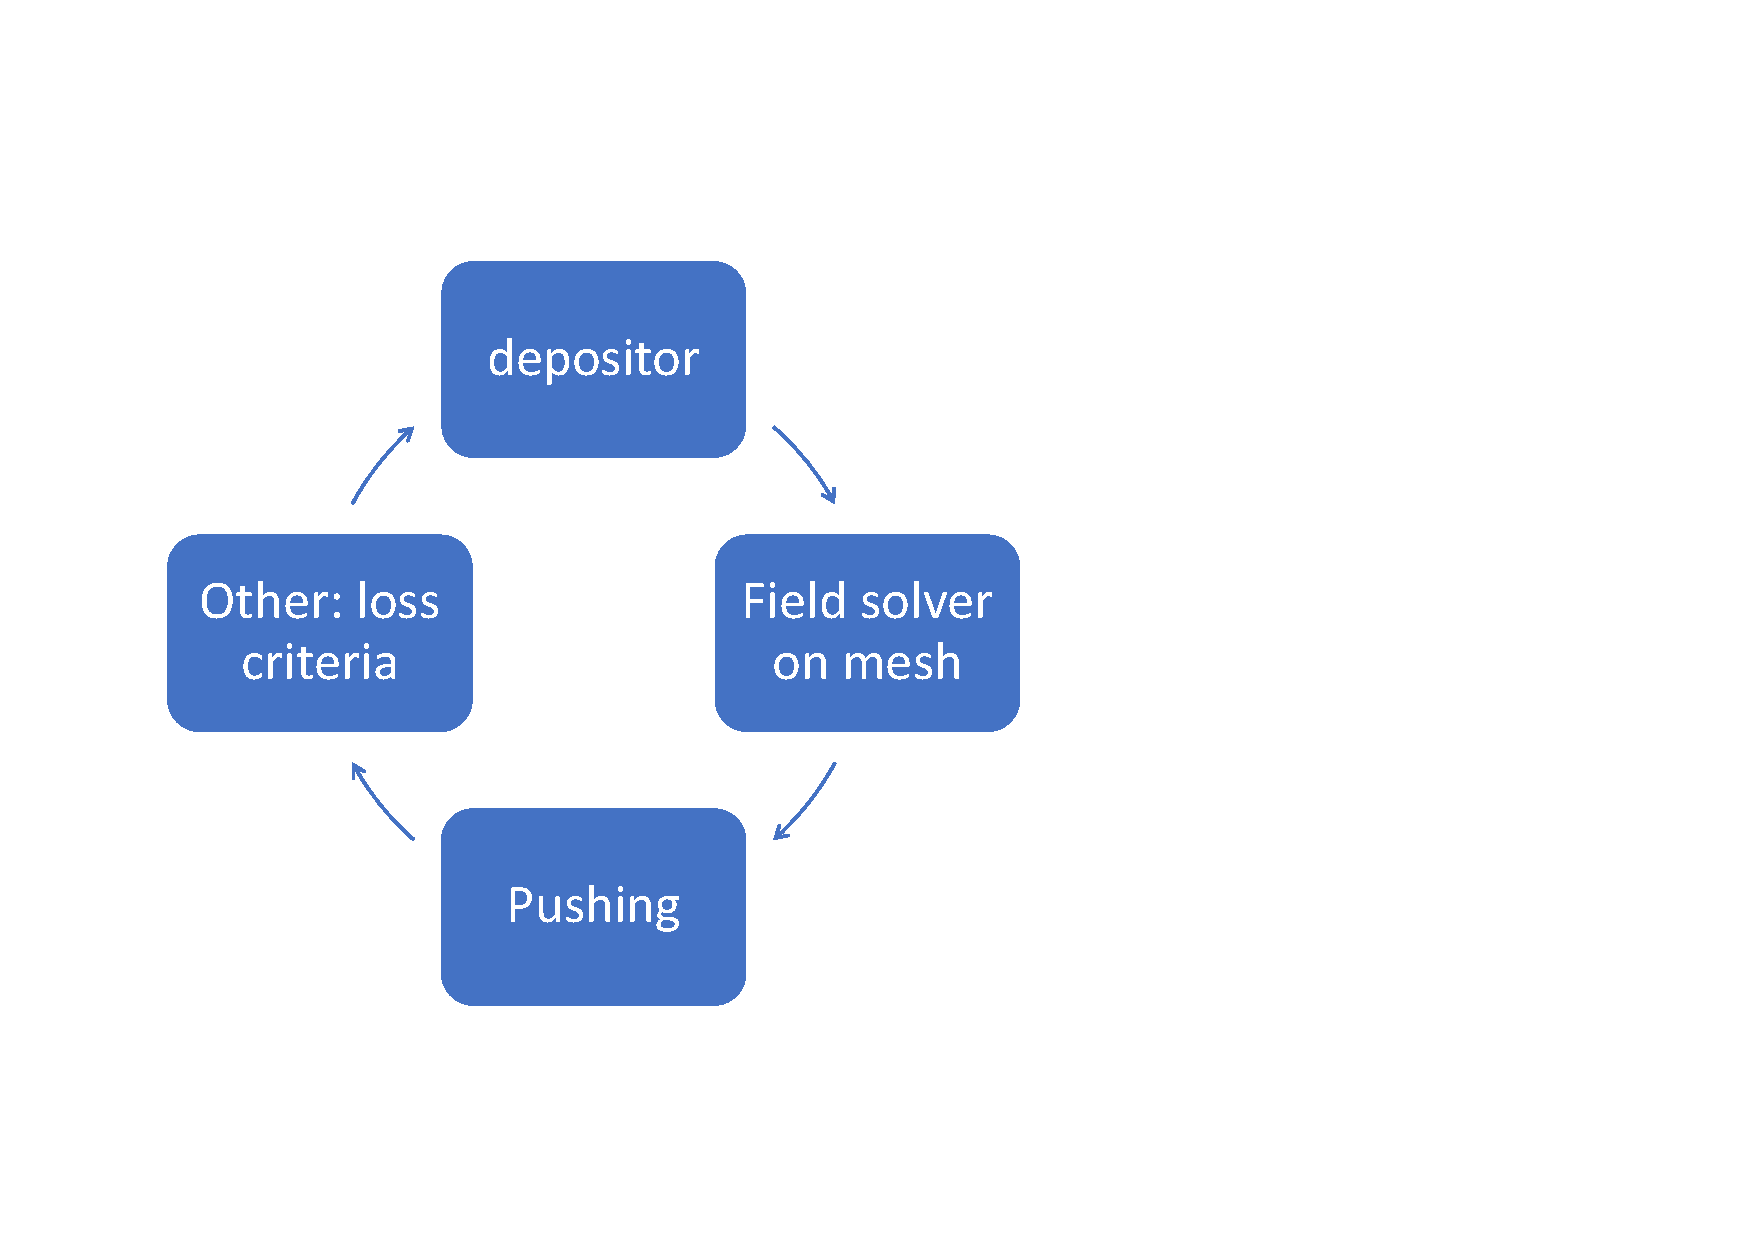
\includegraphics[width=0.6\textwidth]{Img/3_1_PIC.pdf}
    \caption{PIC算法块循环}
    \label{fig:PICflow1}
\end{figure}

\begin{figure}[!tbh]
  \centering
    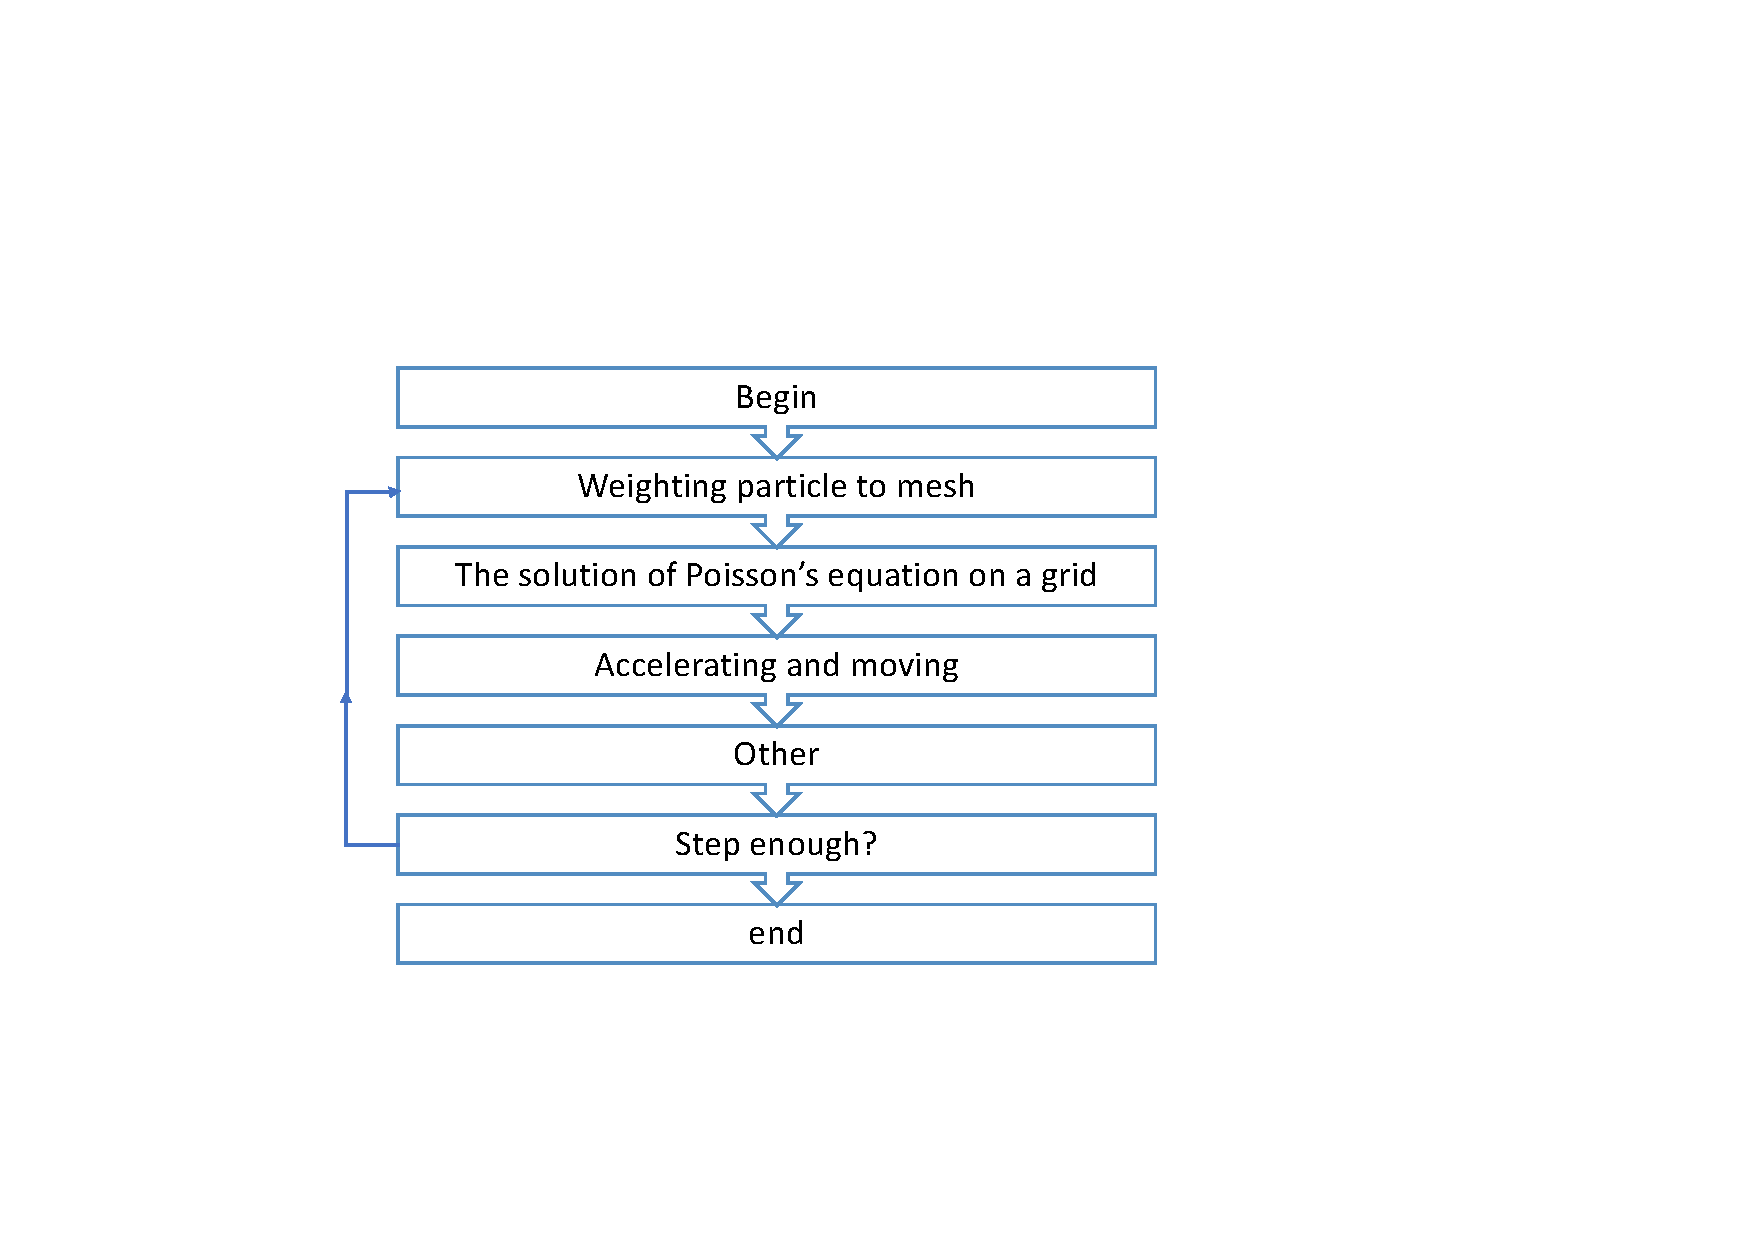
\includegraphics[width=0.7\textwidth]{Img/3_1_PIC2.pdf}
    \caption{PIC算法分段流程}
    \label{fig:PICflow2}
\end{figure}

首先,根据粒子的位置和范围确定所用的空间网格大小,然后执行以下循环:
\begin{enumerate}
  \item 将网格内的所有粒子的电荷根据粒子的位置分配到网格格点上,即从粒子分布得到获得空间点上的密度分布。
  \item 根据网格点上的电荷密度分布,求解网格点上的泊松方程,得到网格点上的电势分布。
  \item 根据电势分布,差分得到网格点上的电场分布。
  \item 根据粒子位置和网格上的电场分布,反向权重得到静止坐标系下粒子所受到的电场,再通过洛伦兹变换得到实验室坐标系下粒子所处位置的电磁场。
  \item 通过牛顿方程,推动粒子,更新粒子位置和动量。
\end{enumerate}

\subsection{权重差值}
PIC算法的第一步是将粒子电荷权重差值到网格上。
粒子权重差值主要有以下几个方面考虑:

\begin{enumerate}
  \item 如何将粒子电荷密度(3D)或者电流密度(2D)权重到空间网格上。
  \item 求解泊松方程后,如何将网格上的电场权重差值回粒子上。
  \item 如何确定网格点的数目和相对于粒子分布的位置及范围。
\end{enumerate}

其中,对于前两个问题,我们最好采用相同的差值算法的正反两个过程,来处理从粒子到网格和从网格到粒子的差值,从而避免算法上带来的非物理效应。如果采用不同的插值方法,可能会出现粒子自己推动自己的错误。

以一维问题为例,将粒子电荷权重到空间网格上的过程,可以理解为粒子坐标$x_i$到网格点上的电荷密度$\rho_p$的一个映射,其中$p$为网格点的坐标。一些常见的权重方法有最近网格点(Nearest Grid Point, NGP),网格云差分法({Cloud In Cell, CIC),三角云分配法(Triangular Shaped Cloud, TSC),如图\ref{fig:PIC_weighting}所示。图中,粒子处于$x$位置,而$p-1,p,p+1$代表不同的网格格点,不同颜色的面积大小代表分配给相应格点的电荷百分比。按照不同的形状分配可以得到不同的结果,
NGP方法为零阶差值,只将电荷分配到离粒子位置最近的网格点上,有较大误差。
CIC方法为一阶差值,根据粒子位置和格点位置的关系,如图\ref{fig:PIC_CIC}所示,将粒子按不同比例分配到临近的两个网格点上。
TSC方法为二阶差值,如图\ref{fig:PIC_TSC}所示,分配函数为三角形,将粒子按不同比例分配到临近的三个网格点上。
\begin{figure}[!htbp]
  \centering
  \begin{subfigure}[b]{0.8\textwidth}
    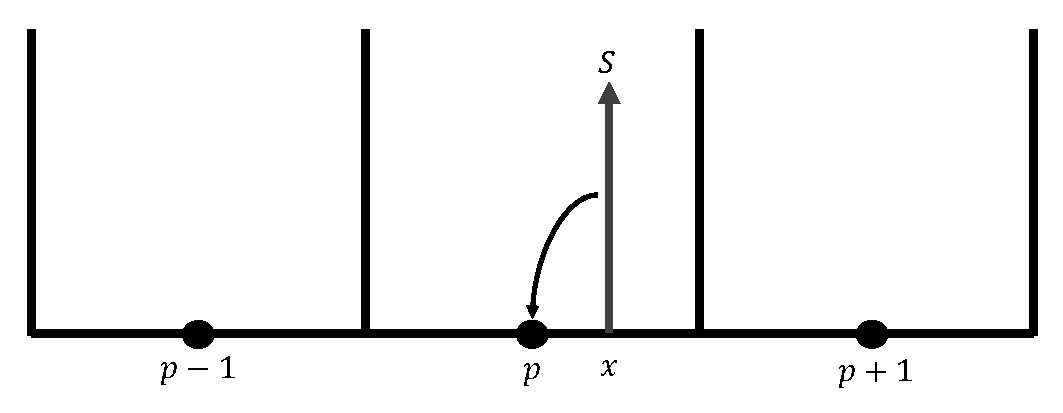
\includegraphics[width=\textwidth]{PIC_NGP}
    \caption{NGP}
    \label{fig:PIC_NGP}
  \end{subfigure}%
  ~%add desired spacing
  \begin{subfigure}[b]{0.8\textwidth}
    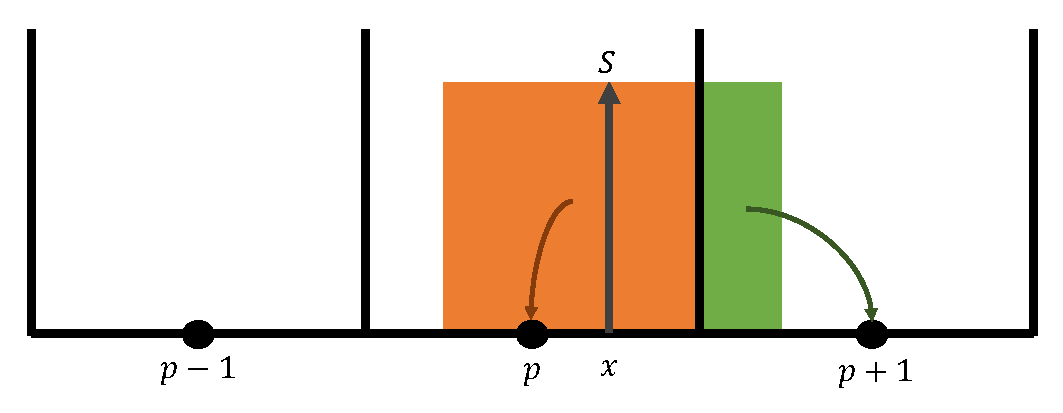
\includegraphics[width=\textwidth]{PIC_CIC}
    \caption{CIC}
    \label{fig:PIC_CIC}
  \end{subfigure}
  \begin{subfigure}[b]{0.8\textwidth}
    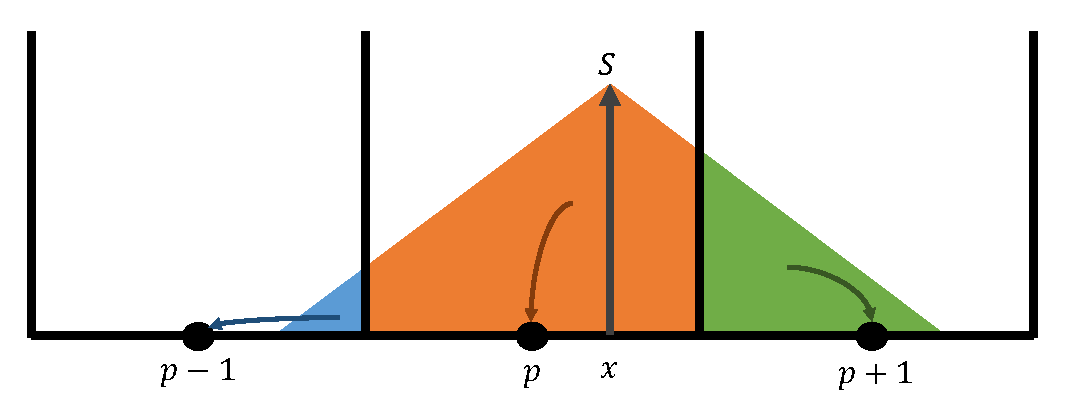
\includegraphics[width=\textwidth]{PIC_TSC}
    \caption{TSC}
    \label{fig:PIC_TSC}
  \end{subfigure}%
  \caption{分配方式示意图}
  \label{fig:PIC_weighting}
\end{figure}

在数学上,这个分配过程可以表示为:
\begin{equation}\label{eq:weight}
  \rho_p=\sum_{i}^{N_p} q_i W(x_i-x_p)
\end{equation}

其中,$q_p$为粒子电荷,$W(x)$为形状因子。如图\ref{fig:PIC_weighting2}所示,根据插值的阶数不同,$W(x)$有很多形式。下式给出了零阶,一阶,和而阶的形状因子:
\begin{equation}\label{eq:NGP}
  S_0(x)=\left\{
  \begin{aligned}
  &1, &\left| x \right| \leqslant \frac{\Delta x}{2} \\
  &0, &\left| x \right| >         \frac{\Delta x}{2}
  \end{aligned}
  \right.
\end{equation}
\begin{equation}\label{eq:CIC}
  S_1(x)=\left\{
  \begin{aligned}
  &1-\frac{\left| x \right|}{\Delta x}, &\left| x \right| \leqslant \Delta x \\
  &0                                  , &\left| x \right| >         \Delta x
  \end{aligned}
  \right.
\end{equation}
\begin{equation}\label{eq:TSC}
  S_2(x)=\left\{
  \begin{aligned}
  &\frac{1}{ \Delta x} \left[\frac{3}{4}-(\frac{\left| x \right|}{\Delta x})^2 \right], &\left| x \right| \leqslant \frac{\Delta x}{2} \qquad \quad \\
  &\frac{1}{2\Delta x} \left[\frac{3}{2}- \frac{\left| x \right|}{\Delta x}    \right], &\frac{\Delta x}{2} < \left| x \right| \leqslant \frac{3\Delta x}{2} \\
  &0,                                                                                   &\left| x \right| > \frac{3\Delta x}{2}\qquad \ \
  \end{aligned}
  \right.
\end{equation}


\begin{figure}[!htbp]
  \centering
  \begin{subfigure}[b]{0.8\textwidth}
    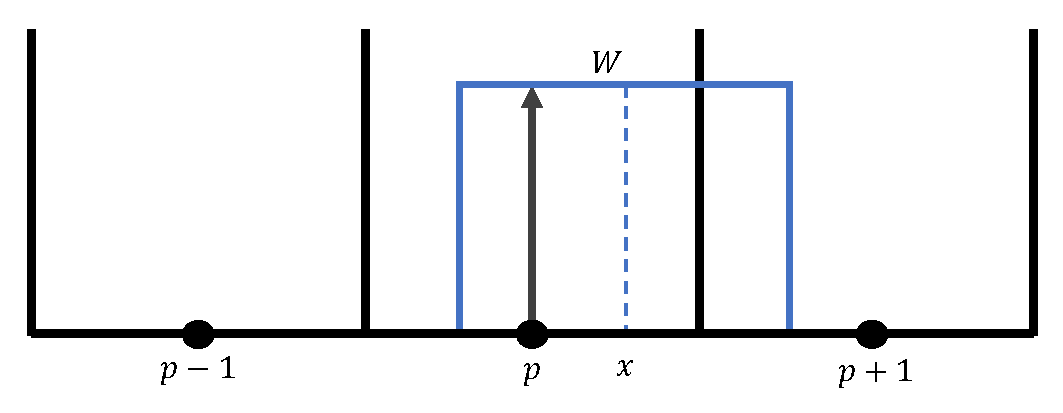
\includegraphics[width=\textwidth]{PIC_NGP2}
    \caption{NGP}
    \label{fig:PIC_NGP2}
  \end{subfigure}%
  ~%add desired spacing
  \begin{subfigure}[b]{0.8\textwidth}
    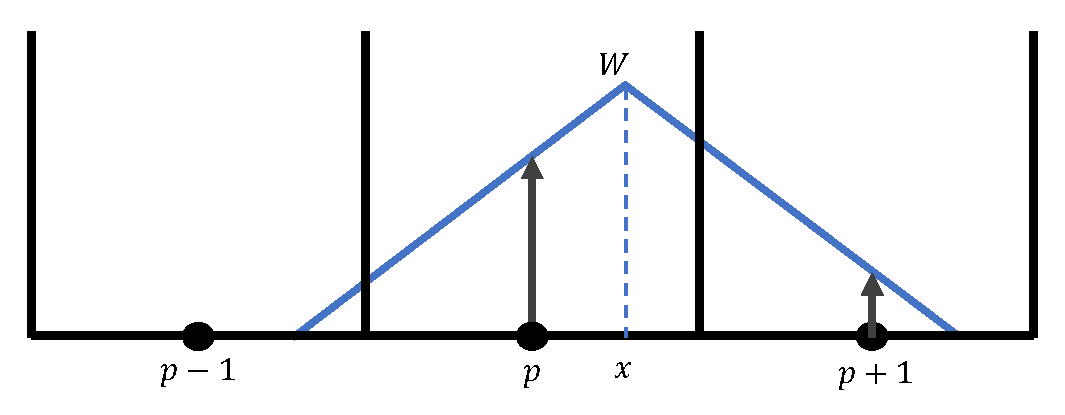
\includegraphics[width=\textwidth]{PIC_CIC2}
    \caption{CIC}
    \label{fig:PIC_CIC2}
  \end{subfigure}
  \begin{subfigure}[b]{0.8\textwidth}
    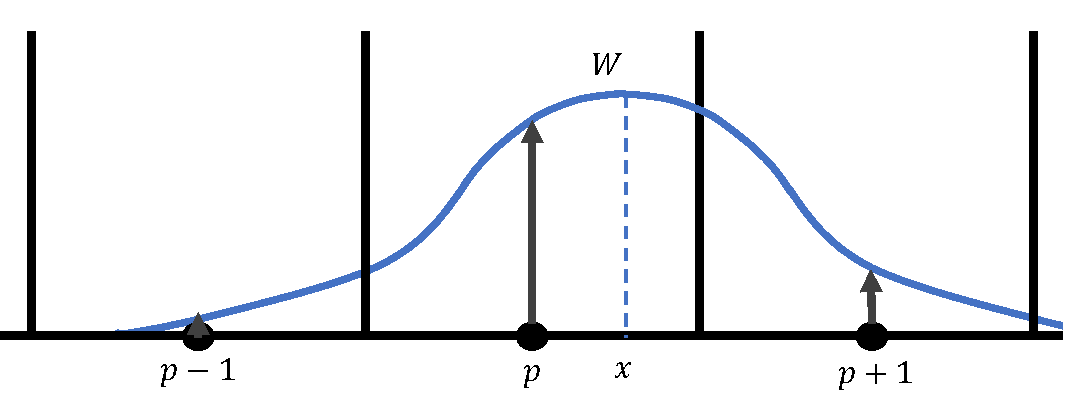
\includegraphics[width=\textwidth]{PIC_TSC2}
    \caption{TSC}
    \label{fig:PIC_TSC2}
  \end{subfigure}%
  \caption{形状因子方程}
  \label{fig:PIC_weighting2}
\end{figure}

在数值模拟中,低阶的算法,比如NGP,会带来很大的粒子离散误差。为了避免数值误差,我们需要采取高阶精度的算法,但是高阶的算法会导致计算量的增大,不满足计算的要求,所以实际中往往采用CIC差值方法。在P-TOPO中,所有的差值形式都采用一阶的线性差值(CIC)。

对于实际的三维问题,处理方法也是类似,我们采用立方网格,使用体积权重法来计算网格上的电荷。

\subsection{使用FFT解泊松方程}
\label{section:PIC_FFT}
经过由粒子到空间网格的权重插值后,我们得到了分布在网格点上的电荷密度分布函数。接下来要做的就是求解网格点上的泊松方程,对于本程序而言,我们使用快速傅里叶变换(FFT)的方法来求解。以一维问题为例,泊松方程:
\begin{equation}\label{eq:Poisson}
\nabla^2 \phi = -\frac{\rho}{\epsilon _0}
\end{equation}
在网格上可以离散表示为:
\begin{equation}\label{eq:PoissonGrid}
\frac{\phi_{j-1}-2\phi_{j}+\phi_{j}}{\Delta _{x}^{2}}=-\frac{\rho _j}{\epsilon _0}
\end{equation}
其中,$\phi_{j}$为第$j$个格点上的电势,$\rho_{j}$为第$j$个格点上的电荷量,$\Delta _{x}$为两个格点之间的距离。

将$\phi_{j}$和$\rho_{j}$进行傅里叶展开,我么可以得到:
\begin{align}
\label{eq:FFT@phi}
\phi _j &= \frac{1}{N_x} \sum_{n=0}^{N_x}{\phi_n \exp{(-\frac{i2 \pi n j}{N_x} )}} \\
\label{eq:FFT@rho}
\rho _j &= \frac{1}{N_x} \sum_{n=0}^{N_x}{\rho_n \exp{(-\frac{i2 \pi n j}{N_x} )}}
\end{align}
其中,$N_x$为一个方向上网格点的数目。

将式\ref{eq:FFT@phi}和式\ref{eq:FFT@rho}代回式\ref{eq:PoissonGrid}可得:
\begin{equation}\label{eq:FFT@PIC2}
\begin{aligned}
\sum_{n=0}^{N_x}{\phi_n
\left(\exp{(-\frac{i2 \pi n (j-1)}{N_x} )}  -2\exp{(-\frac{i2 \pi n j}{N_x} )}  +  \exp{(-\frac{i2 \pi n (j+1)}{N_x} )}\right)} \\
= \frac{\Delta _{x}^{2}}{\epsilon _0} \sum_{n=0}^{N_x}{\rho_n \exp{(-\frac{i2 \pi n j}{N_x} )}} \qquad\qquad\qquad
\end{aligned}
\end{equation}

对于傅里叶空间的的电势和电荷密度,我们可以得到$\phi_{n}$和$\rho_{n}$的关系:
\begin{equation}\label{eq:FFT@PIC3}
\phi_{n}\left(\exp{(\frac{i2 \pi n}{N_x} )}  +  \exp{(-\frac{i2 \pi n}{N_x})} - 2 \right)
 = \frac{\Delta _{x}^{2}}{\epsilon _0} {\rho_n} \\
\end{equation}
化简得到
\begin{equation}\label{eq:FFT@PIC3}
\phi_{n} = \frac{\rho_n}{\epsilon _0 K_n^2} \\
\end{equation}
其中
\begin{equation}\label{eq:FFT@PIC4}
K_n = (\frac{2\pi n}{N_x \Delta _x}) \frac{\sin({\pi n}/{N_x})}{{\pi n}/{N_x}} \\
\end{equation}

可以看出,通过傅里叶变换得到的傅里叶空间中的电荷密度$\rho_{n}$,我们可以得到傅里叶空间中的电势分布函数$\phi_{n}$。然后再经过傅里叶逆变换,我们就可以得到是空间中的电势分布$\phi_{j}$,最后经过差分我们就可以得到空间电场分布函数。如图\ref{fig:PIC_FFT_Poisson}所示:
\begin{figure}[ht]
  \begin{equation*}
    \centering
    \rho_j \quad \xrightarrow{FFT} \quad \rho_n  \quad \xrightarrow{Multuply\ by\ \frac{1}{K_n^2}}   \quad  \phi_n  \quad \xrightarrow{IFFT} \quad  \phi_j \quad \xrightarrow{Finite\ Difference} \quad  E_{x,j}
  \end{equation*}
  \caption{使用FFT求解泊松方程}
  \label{fig:PIC_FFT_Poisson}
\end{figure}

需要注意的是,这种$\exp$指数的傅里叶变换方式决定了我们使用的是周期性边界条件。如果我们想要第一类边界条件,我们需要采用$\sin$函数变换,其变换过程与FFT类似。
在本程序中,我们在横向采用第一类边界条件,用来模拟边界处的电势为0;而在纵向采用周期性边界条件,用以模拟连续束流。

\subsection{使用蛙跳法推动粒子}

我们使用经典的牛顿方程来推动粒子:
\begin{align}
\label{eq:PIC_push1}
 \frac{\mathrm{d} \mathbf{x}}{\mathrm{d} t} &= \mathbf{v}  \\
\label{eq:PIC_push2}
m\frac{\mathrm{d} \mathbf{v}}{\mathrm{d} t} &= \mathbf{F}
\end{align}
粒子推动的方法必须满足以下五个条件:
\subsubsection{一致性}
      一致性是指差分方程和微分方程的一致。任何数值算法都是使用有限大小的步长来模拟一个连续的过程。
      因此,我们我们应该在时间步长无线小的时候,使其效果与连续推动一致。

      例如,我们采用有限步长$\Delta T$ 来推动粒子位置:
      \begin{align}
         \label{eq:PIC_push3}
         \frac{\mathbf{x}_{n+1}-\mathbf{x}_n}{\Delta T} &= \mathbf{v}_n  \\
         \label{eq:PIC_push4}
          m\frac{\mathbf{v}_{n+1}-\mathbf{v}_n}{\Delta T} &= \mathbf{F}_n
      \end{align}
                当其步长$\Delta T$足够小时,其结果应该与微分方程\ref{eq:PIC_push1} 和\ref{eq:PIC_push2}相一致。
\subsubsection{同时性}
      同时性又叫做可逆性。微分方程\ref{eq:PIC_push1}和\ref{eq:PIC_push2}是可逆的。例如,一个粒子在给定的力场中沿时间正向积分运动,然后如果将其速度取反,并沿时间反向积分,粒子将会沿着正向的轨迹向回运动,并能回到起始点。

      这一点在差分近似中并不能得到保证,比如,差分方程\ref{eq:PIC_push3}和\ref{eq:PIC_push4}中,粒子在第$n+1$步处取反,粒子位置变化为
      \begin{equation}
         \label{eq:PIC_push5}
         \frac{\mathbf{x}_{n}-\mathbf{x}_{n+1}}{\Delta T} = -\mathbf{v}_{n+1}
      \end{equation}
      其速度为$\mathbf{v}_{n+1}$而不是$\mathbf{v}_{n}$,也就是说粒子并不能沿其轨迹回到初始位置。这是因为差分方程的左右的时间中心不相同,式\ref{eq:PIC_push3}左侧,位置改变为$\mathbf{x}_{n+1}-\mathbf{x}_n$,是以$t_{n+1/2}$为时间中心的;而右侧$\mathbf{v}_n$是时间$t_{n}$ 时的速度。因此,我们需要将其改变为:
      \begin{align}
         \label{eq:PIC_push6}
         \frac{\mathbf{x}_{n+1}-\mathbf{x}_n}{\Delta T} &= \mathbf{v}_{n+1/2}  \\
         \label{eq:PIC_push7}
          m\frac{\mathbf{v}_{n+1/2}-\mathbf{v}_{n-1/2}}{\Delta T} &= \mathbf{F}_n
      \end{align}
      这也就是蛙跳法,即位置的时间与速度的时间并不在统一时刻,而是采用相差半个步长,然后交替推动粒子的速度和位置,以满足同时性条件。
\subsubsection{准确性}

      准确性与一步计算中的数值解与解析解的误差有关。这个误差主要来源于两方面:第一,来自于计算机的精度,例如,双精度浮点数仅有十四或十五位有效数字;第二,来自于使用有限小的步长代表连续变量的截断误差。通常来讲,第一种来自计算机数值精度的误差非常小,如果算法是稳定的(关于稳定性的论述见下一条),这个误差是可以忽略的。第二种来自于有限小的步长的误差,可以由解析解与数值解的差值来表示,其差值通常与步长$\Delta T$的$n$ 次方$(\Delta T)^n$的成正比,而不同算法之间的稳定性可由阶数$n$来表示。

      由式\ref{eq:PIC_push6}和\ref{eq:PIC_push7} 可知,蛙跳法为解析解\ref{eq:PIC_push1}和\ref{eq:PIC_push2}的二阶近似。证明如下:由式\ref{eq:PIC_push6} 和\ref{eq:PIC_push7}可得:
      \begin{equation}
         \label{eq:leapfrog_accuracy}
         \frac{\mathbf{x}_{n+1}-2\mathbf{x}_{n}+\mathbf{x}_{n-1}}{(\Delta T)^2} = \frac{\mathbf{F}(\mathbf{x}_n)}{m}
      \end{equation}
      如果$\mathbf{X}$为解析解:
      \begin{equation}
         \label{eq:leapfrog_accuracy2}
         \frac{\mathrm{d}^2 \mathbf{X}}{\mathrm{d} t^2} = \frac{\mathbf{F}}{m}
      \end{equation}
      那么有限小步长的误差可以由${\delta}^n$表示:
      \begin{equation}
         \label{eq:leapfrog_accuracy3}
         \frac{\mathbf{X}_{n+1}-2\mathbf{X}_{n}+\mathbf{X}_{n-1}}{(\Delta T)^2} = \frac{\mathbf{F}(\mathbf{X}_n)}{m} - {\delta}^n
      \end{equation}
      将$\mathbf{X}_{n+1}$和$\mathbf{X}_{n-1}$泰勒在$\mathbf{X}_{n}=\mathbf{X}(t_n)$ 处展开,式\ref{eq:leapfrog_accuracy3}可以写作:
      \begin{equation}
         \label{eq:leapfrog_accuracy4}
         \frac{\mathrm{d}^2 \mathbf{X}}{\mathrm{d} t^2} + \frac{(\Delta T)^2}{12} \frac{\mathrm{d}^4 \mathbf{X}}{\mathrm{d} t^4} + h.o.t. =  \frac{\mathbf{F}(\mathbf{X}_n)}{m} - {\delta}^n
      \end{equation}
      其中 $h.o.t.$ 为高阶项(high order term)。式\ref{eq:leapfrog_accuracy3} 与式\ref{eq:leapfrog_accuracy4}相减可得:
      \begin{equation}
         \label{eq:leapfrog_accuracy5}
         {\delta}^n = -\frac{(\Delta T)^2}{12} \frac{\mathrm{d}^4 \mathbf{X}}{\mathrm{d} t^4} + h.o.t.
      \end{equation}
      即,蛙跳法为二阶准确度(${\delta}^n \propto (\Delta T)^2$)。
\subsubsection{稳定性}
稳定性与误差随时间的变化有关。即使算法每一步的误差非常小,最终误差也有可能由于累积效应导致变大。
在一个数值算法中,如果每一步的误差不会导致一个更大的累积误差,那么这个算法是稳定的。

下面,我们讨论蛙跳法的稳定性。根据式\ref{eq:leapfrog_accuracy},如果我们给定$\mathbf{x}_0 = \mathbf{X}_0,\mathbf{x}_1 = \mathbf{X}_1$作为初始条件,不考虑误差的情况下,我们可以得到之后的一系列解$\mathbf{X}_2,\mathbf{X}_3,\mathbf{X}_4,...$,其中:
      \begin{align}
         \label{eq:leapfrog_stability1}
         \mathbf{X}_{2}-2\mathbf{X}_{1}+\mathbf{X}_{0} &= \frac{\mathbf{F}(\mathbf{X}_1)}{m} {(\Delta T)^2} \\
         \label{eq:leapfrog_stability2}
         \mathbf{X}_{3}-2\mathbf{X}_{2}+\mathbf{X}_{1} &= \frac{\mathbf{F}(\mathbf{X}_2)}{m} {(\Delta T)^2}
      \end{align}

然而,由于误差存在,我们无法得到微分方程中的精确解$\mathbf{X}_2,\mathbf{X}_3,\mathbf{X}_4,...$,而是会得到一系列含有误差近似解$\mathbf{x}_2,\mathbf{x}_3,\mathbf{x}_4,...$:
      \begin{align}
         \label{eq:leapfrog_stability3}
         \mathbf{x}_{2}-2\mathbf{X}_{1}+\mathbf{X}_{0} &= \frac{\mathbf{F}(\mathbf{X}_1)}{m} {(\Delta T)^2} \\
         \label{eq:leapfrog_stability4}
         \mathbf{x}_{3}-2\mathbf{x}_{2}+\mathbf{X}_{1} &= \frac{\mathbf{F}(\mathbf{X}_2)}{m} {(\Delta T)^2}
      \end{align}

如此,在第二步处的误差为:
      \begin{equation}
         \label{eq:leapfrog_stability5}
         {\epsilon}_2 = \mathbf{x}_2 -\mathbf{X}_2
      \end{equation}

在随后的每一步计算中,含有误差的近似结果都会被使用,我们需要知道的是${\epsilon}_2$是如何影响后续计算结果。由式\ref{eq:leapfrog_stability3}和式\ref{eq:leapfrog_stability4}可得:
      \begin{equation}
         \label{eq:leapfrog_stabilit6}
         (\mathbf{X}_{3}+{\epsilon}_3)-2(\mathbf{X}_{x}+{\epsilon}_2)+\mathbf{X}_{1} = \frac{\mathbf{F}(\mathbf{X}_2+{\epsilon}_2)}{m} {(\Delta T)^2}
      \end{equation}
与式\ref{eq:leapfrog_stability2}相比较,可得:
      \begin{equation}
         \label{eq:leapfrog_stabilit7}
         {\epsilon}_3-2{\epsilon}_2 = \left(\mathbf{F}(\mathbf{X}_2+{\epsilon}_2)  -\mathbf{F}(\mathbf{X}_2) \right)\frac{{(\Delta T)^2}}{m}
      \end{equation}
将上式右侧在$\mathbf{x}=\mathbf{X}^2$处进行泰勒展开:
      \begin{equation}
         \label{eq:leapfrog_stabilit8}
         {\epsilon}_3-2{\epsilon}_2 \approx {\epsilon}_2\left. \frac{\partial\mathbf{F}}{\partial\mathbf{x}}\right|_{\mathbf{x}=\mathbf{X}^2} \frac{{(\Delta T)^2}}{m}
      \end{equation}
类似可得:
      \begin{equation}
         \label{eq:leapfrog_stabilit9}
         {\epsilon}_4-2{\epsilon}_3+{\epsilon}_2 = {\epsilon}_3\left. \frac{\partial\mathbf{F}}{\partial\mathbf{x}}\right|_{\mathbf{x}=\mathbf{X}^3} \frac{{(\Delta T)^2}}{m}
      \end{equation}
则第n步的误差为:
      \begin{equation}
         \label{eq:leapfrog_stabilit10}
         {\epsilon}_{n+1}-2{\epsilon}_n+{\epsilon}_{n-1} = {\epsilon}_n \left. \frac{\partial\mathbf{F}}{\partial\mathbf{x}}\right|_{\mathbf{x}=\mathbf{X}^n} \frac{{(\Delta T)^2}}{m}
      \end{equation}
上式并不能得到一个准确的误差递进关系,除非${\partial\mathbf{F}}/{\partial\mathbf{x}}$为常量。由于我们的目标是判断算法是否稳定,而不是算法有多稳定,所以我们考虑最坏的情况,使用$-|{\partial\mathbf{F}}/{\partial\mathbf{x}}|_{max}$代替${\partial\mathbf{F}}/{\partial\mathbf{x}}$,其中的负号是因为我们假设所计算的问题是有限边界,而不是会延伸到无穷远。可得误差随时间的变化方程:
      \begin{align}
         \label{eq:leapfrog_stabilit11}
         {\epsilon}_{n+1}-2{\epsilon}_n+{\epsilon}_{n-1} &= -\left| \frac{\partial\mathbf{F}}{\partial\mathbf{x}}\right|_{max} \frac{{(\Delta T)^2}}{m} {\epsilon}_n \\
         {\epsilon}_{n+1}-2{\epsilon}_n+{\epsilon}_{n-1} &= -(\Omega \Delta T)^2 {\epsilon}_n
         \label{eq:leapfrog_stabilit12}
      \end{align}
其解的形式与震荡方程形式类似${\epsilon}_n = {\lambda}_n = \exp(i\omega n \Delta T)$。两个特征解${\lambda}_+$和${\lambda}_-$为:
      \begin{equation}
         \label{eq:leapfrog_stabilit13}
         {\lambda}_\pm = 1- \frac{(\Omega \Delta T)^2}{2}\pm \left[\frac{(\Omega \Delta T)^2}{2}\right]\left[1-\frac{4}{(\Omega \Delta T)^2}\right]^{1/2}
      \end{equation}
对于算法而言,想要保证数值上稳定,其误差不能随着时间而变大,即误差推动方程的特征解必须位于单位圆内,即$|\lambda|\leq1$。

因此,我们必须使时间步长足够小,才能保证算法稳定,对于蛙跳法而言,我们必须使:
      \begin{equation}
          \Omega \Delta T \leq 2
      \end{equation}
%\subsection{效率}
%blabla...


\section{Symplectic算法}
\label{section:symplectic_theory}

PIC算法是求解空间电荷效应非常快速有效的方法,在PIC算法中,粒子首先被根据位置权重到网格上,然后根据网格上的电荷密度求解泊松方程,得到网格上的电势,从而得到网格上的电场,再根据粒子位置反推出粒子所处位置的电场。使用这种方法,计算复杂度由直接的粒子-粒子方法的 $N_p^2$ 降低到了$\alpha N_p + \beta N_{cells}\log{N_{cells}}$。其中 $N_p$ 是粒子数,而$N_{cells}$ 是网格点数目。

然而,由于PIC算法不可避免的会带来网格热噪声,因此目前加速器界常用的PIC算法并不能保障辛条件(symplectic)。其计算就会被引入非物理效应,并对最终的强流束流物理的分析和讨论会带来一些干扰。因此,在需要长程模拟(比如环形加速器)的物理分析中,我们需要一种保辛的算法。

最初,保辛算法本身是为了保障哈密顿系统中的辛条件而被研究 \cite{symplectic_channel1990, symplectic_yoshida1990}。最近,无网格保辛模型被引入到加速器研究中作为空间电荷求解器 \cite{symplectic_ji2017}。
这种模型并不利用网格,而是利用高阶分解来求解空间电荷效应。
相比PIC算法,这种方法能够显著的降低由于网格数值噪声带来的发射度增长。
然而,虽然能够保证辛条件,这种算法也有缺陷,最显著的就是计算量要大得多。
无网格算法的计算复杂度为 $\alpha N_p * N_{modes}$ ,其中$N_{modes}$为分解的阶数,在通常模拟中我们一般使用$16 \times 16 \times 16$ 阶,在这种配置下花费的时间比PIC算法要高两到三个数量级。
所以我们必须提高这个算法的运行速度,以提高算法的实用性。
幸运的是,由于无网格算法很适合并行的特性,这种算法能够很好的被加速,并且有很好的可扩展性。
下面,我们简要介绍保辛算法的基本原理。

在束流动力学模拟中,当且仅当雅可比矩阵$M_i$满足以下条件时,传输矩阵$ m_i $才是保辛的\cite{accelerator2004lee, accelerator2013chao}:
\begin{equation}
M_{i}^{T}J{{M}_{i}}=J
\end{equation}
其中,$J$ 是如下 $6N\times6N$ 的矩阵:
\begin{equation}
J=\left(
  \begin{array}{cc}
     0 & I \\
    -I & 0 \\
  \end{array}
\right)
\end{equation}

对于考虑其空间电荷力的多粒子系统,哈密尔顿量可以写为:
\begin{equation}
H={{H}_{1}}+{{H}_{2}}
\end{equation}
其中
\begin{eqnarray}
% \nonumber to remove numbering (before each equation)
  {H}_{1} &=& \sum\limits_{i}{{p_{i}^{2}}/{2}\;}+\sum\limits_{i}{q\psi ({{r}_{i}})} \\
  {H}_{2} &=& \frac{1}{2}\sum\limits_{i}{\sum\limits_{j}{q\varphi ({{r}_{i}},{{r}_{j}})}}
\end{eqnarray}

其中${{H}_{1}}$ 只包含外场信息,而 ${{H}_{2}}$ 只包括空间电荷效应。根据${{H}_{1}}$ 和 ${{H}_{2}}$ 得到的两个传输矩阵 ${{m}_{1}}$和 ${{m}_{2}}$,一个二阶传输矩阵$m\left( \tau  \right)$可以被定义为:
\begin{equation}
m\left( \tau  \right)={{m}_{1}}\left( \tau /2 \right){{m}_{2}}\left( \tau  \right){{m}_{1}}\left( \tau /2 \right)
\end{equation}

如果$ {{m} _ {1}} $和$ {{m} _ {2}} $都是保辛的,那么$ m $就是保辛的。在大多数加速器元件中,我们可以通过单粒子动力学获得相应的外场传输矩阵$ {{m} _ {1}} $,而内场传输矩阵$ {{m} _ {2}} $可以写为:
\begin{eqnarray}
 {{r}_{i}}(\tau ) &=& {{r}_{i}}(0) \\
 {{p}_{i}}(\tau ) &=& {{p}_{i}}(0)-\frac{\partial {{H}_{2}}(r)}{\partial {{r}_{i}}}\tau
\end{eqnarray}
其雅克比矩阵为:
\begin{equation}
{{M}_{2}}=\left(
\begin{array}{cc}
   I & 0  \\
   L & I  \\
\end{array} \right)
\end{equation}
其中
${{L}_{ij}}=\frac{\partial {{p}_{i}}(\tau )}{\partial {{r}_{j}}}=-\frac{{{\partial }^{2}}{{H}_{2}}(r)}{\partial {{r}_{i}}\partial {{r}_{j}}}\tau$
是一个对称矩阵,所以${{M}_{2}}$满足保辛条件.

对于一个3D束团, ${{H}_{2}}$可以表示为:
\begin{equation}
{{H}_{2}}=\kappa {{\gamma }_{0}}\sum\limits_{i}{\sum\limits_{j}{\varphi ({{r}_{i}},{{r}_{j}})}}
\end{equation}
其中 $\kappa =q/(lm{{C}^{2}}\gamma _{0}^{2}{{\beta }_{0}}),l=C/\omega $。而在束流坐标系下的静电势可以有泊松方程得到:
\begin{equation}
\frac{{{\partial }^{2}}\phi }{\partial {{x}^{2}}}+\frac{{{\partial }^{2}}\phi }{\partial {{y}^{2}}}+\frac{{{\partial }^{2}}\phi }{\partial {{z}^{2}}}=-\frac{\rho }{{{\varepsilon }_{0}}}
\end{equation}
其中边界条件为:
\begin{equation}
\begin{array}{cc}
   \phi (x=0,y,z)=0, & \phi (x=a,y,z)=0  \\
   \phi (x,y=0,z)=0, & \phi (x,y=b,z)=0  \\
   \phi (x,y,z=0)=0, & \phi (x,y,z=c)=0  \\
\end{array}
\end{equation}
其中,$a$,$b$,$c$分别是X,Y,Z方向上的零电势边界长度。如果我们将$c$设的足够大,电势将在无穷远处为零。

泊松方程中的电势$\phi$和电荷密度$\rho$可以展开为:
\begin{eqnarray}
 \rho(x,y,z)&=&\sum\limits_{l=1}^{{{N}_{l}}}{\sum\limits_{m=1}^{{{N}_{m}}}{\sum\limits_{n=1}^{{{N}_{n}}}{{{\rho }^{lmn}}\sin ({{\alpha }_{l}}x)\sin ({{\beta }_{m}}y)\sin ({{\gamma }_{n}}z)}}} \\
 \phi(x,y,z)&=&\sum\limits_{l=1}^{{{N}_{l}}}{\sum\limits_{m=1}^{{{N}_{m}}}{\sum\limits_{n=1}^{{{N}_{n}}}{{{\phi }^{lmn}}\sin ({{\alpha }_{l}}x)\sin ({{\beta }_{m}}y)\sin ({{\gamma }_{n}}z)}}}
\end{eqnarray}
其中 ${N}_{l}$,${N}_{m}$,${N}_{n}$分别为电势和电荷密度在X,Y,Z三个方向上展开的阶数,而 ${\rho }^{lmn}$和 ${\phi }^{lmn}$可以表达为:
\begin{eqnarray}
  {{\rho }^{lmn}}&=&\frac{8}{abc}\int\limits_{0}^{a}{\int\limits_{0}^{b}{\int\limits_{0}^{b}{\rho (x,y,z)\sin ({{\alpha }_{l}}x)\sin ({{\beta }_{m}}y)\sin ({{\gamma }_{n}}z)dxdydz}}} \\
 {{\phi }^{lmn}}&=&\frac{8}{abc}\int\limits_{0}^{a}{\int\limits_{0}^{b}{\int\limits_{0}^{b}{\phi (x,y,z)\sin ({{\alpha }_{l}}x)\sin ({{\beta }_{m}}y)\sin ({{\gamma }_{n}}z)dxdydz}}}
\end{eqnarray}
其中
\begin{equation}
{{\alpha }_{l}}=\frac{l\pi }{a},{{\beta }_{m}}=\frac{m\pi }{b},{{\gamma }_{n}}=\frac{n\pi }{c}
\end{equation}

将上面的展开代入泊松方程,我们可以得到:
\begin{equation}
{{\phi }^{lmn}}=\frac{{{\rho }^{lmn}}}{{{\varepsilon }_{0}}(\alpha _{l}^{2}+\beta _{m}^{2}+\gamma _{n}^{2})}
\end{equation}

据此,我们得到了粒子密度$ \ rho $和电势$ \ phi $之间的关系:
\begin{multline}
\phi (x,y,z)=\frac{1}{{{\varepsilon }_{0}}}\frac{8}{abc}\omega \times \\ \sum\limits_{j=1}^{{{N}_{j}}}{\sum\limits_{l=1}^{{{N}_{l}}}{\sum\limits_{m=1}^{{{N}_{m}}}{\sum\limits_{n=1}^{{{N}_{n}}}{\frac{\sin ({{\alpha }_{l}}{{x}_{j}})\sin ({{\beta }_{m}}{{y}_{j}})\sin ({{\gamma }_{n}}{{z}_{j}})\sin ({{\alpha }_{l}}x)\sin ({{\beta }_{m}}y)\sin ({{\gamma }_{n}}z)}{(\alpha _{l}^{2}+\beta _{m}^{2}+\gamma _{n}^{2})}}}}}
\end{multline}
其中 $\omega $ 是粒子的电荷。

于是哈密顿量 ${{H}_{2}}$可以表示为:
\begin{multline}
{{H}_{2}}=\frac{1}{{{\varepsilon }_{0}}}\frac{8}{abc}\omega \kappa {{\gamma}_{0}} \times \\
\sum\limits_{i=1}^{{{N}_{i}}}{\sum\limits_{j=1}^{{{N}_{j}}}{\sum\limits_{l=1}^{{{N}_{l}}}{\sum\limits_{m=1}^{{{N}_{m}}}{\sum\limits_{n=1}^{{{N}_{n}}}
{\frac{\sin ({{\alpha }_{l}}{{x}_{j}})\sin ({{\beta }_{m}}{{y}_{j}})\sin ({{\gamma }_{n}}{{z}_{j}})\sin ({{\alpha }_{l}}{{x}_{i}})\sin ({{\beta }_{m}}{{y}_{i}})\sin ({{\gamma }_{n}}{{z}_{i}})}{(\alpha _{l}^{2}+\beta _{m}^{2}+\gamma _{n}^{2})}}
}}}}
\end{multline}

我们得到了保辛的空间电荷传输矩阵 ${{m}_{2}}$。 以X方向为例:
\begin{align}
&{{x}_{i}}(\tau )= {{x}_{i}}(0) \\
 \nonumber &{{p}_{xi}}(\tau )= {{p}_{xi}}(0)-\tau \frac{1}{{{\varepsilon }_{0}}}\frac{8}{abc}\omega \kappa {{\gamma }_{0}} \times \\
 &\sum\limits_{j=1}^{{{N}_{j}}}{\sum\limits_{l=1}^{{{N}_{l}}}{\sum\limits_{m=1}^{{{N}_{m}}}{\sum\limits_{n=1}^{{{N}_{n}}}{\frac{{{\alpha }_{l}}\sin ({{\alpha }_{l}}{{x}_{j}})\sin ({{\beta }_{m}}{{y}_{j}})\sin ({{\gamma }_{n}}{{z}_{j}})\cos ({{\alpha }_{l}}{{x}_{i}})\sin ({{\beta }_{m}}{{y}_{i}})\sin ({{\gamma }_{n}}{{z}_{i}})}{(\alpha _{l}^{2}+\beta _{m}^{2}+\gamma _{n}^{2})}}}}}\label{eq:map1}
\end{align}
在Y和Z方向的传输矩阵与之类似。


\section{GPU和CPU架构}
GPU英文全称Graphic Processing Unit,中文为“图形处理器”。
GPU一开始是由于在现代的计算机中图形的处理变得越来越重要,需要一个专门的图形的核心处理器,使显卡减少对CPU的依赖,并进行部分原本CPU的工作;CPU是英文全称为Central Processing Unit,中文为“中央处理器”,一般由逻辑运算单元、控制单元和存储单元组成。
近年来,GPU高速发展,极大的提高了计算机图形处理的速度和质量,不但促进了图像处理、虚拟现实、计算机仿真等相关应用领域的快速发展,同时也为人们利用GPU进行图形处理以外的通用计算提供了良好的运行平台。

相对于CPU,GPU在并行处理和计算密集型问题方面具有很大优势。目前,GPU已成为普通计算机强大、高效的计算资源。如图\ref{fig:GPU}所示,一个CPU一般只拥有少数几个核,而一个GPU会有几百甚至几千个核。从系统架构上看,GPU针对向量计算进行了高度并行的数据流优化处理,这种多核架构特别适合进行数据并行。这种以数据流作为处理单元的机制,在对数据流的处理上可以取得很高的速度。
GPU 加速计算是指同时利用GPU 和 CPU,加快应用程序的运行速度\cite{gpu2008}。GPU厂商为科学计算设计了自己的API,其中CUDA(Compute Unified Device Architecture)就是NVIDIA设计的并行计算平台和编程规范\cite{nvidia2010programming}。利用CUDA,我们能够有效的利用GPU,使程序的运行效率大大提高。

根据使用CUDA的测试结果显示,利用GPU实现FFT(Fast Fourier Transformation)、BLAS(Basic Linear Algebra Subprograms)、排序及线性方程组求解等科学计算,与单纯依靠CPU实现的算法相比,平均性能提高了近20倍。
\begin{figure}[!htb]
    \centering
    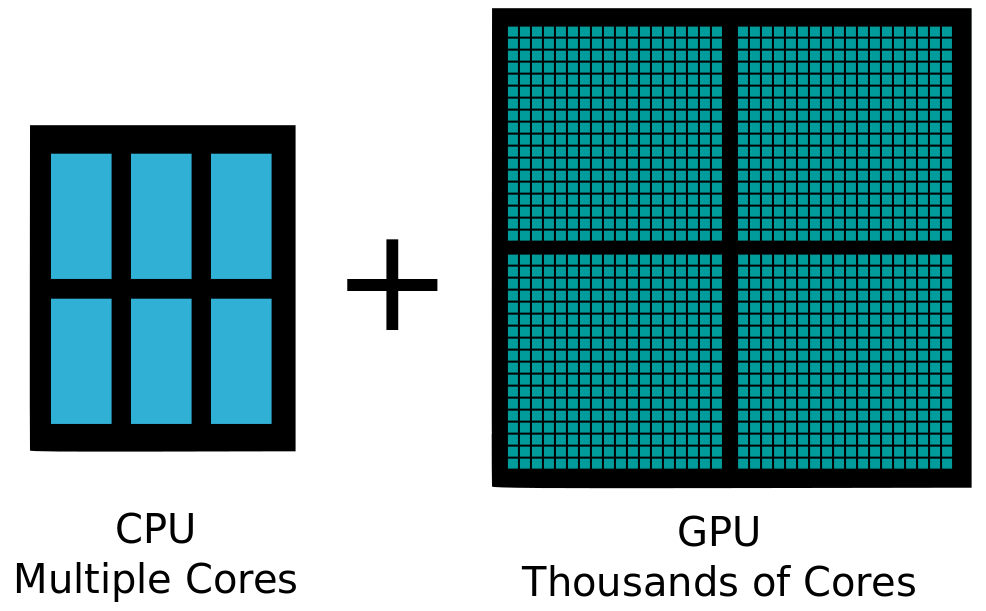
\includegraphics[width=0.9\textwidth]{plot/GPU_vs_CPU.png}
    \caption{GPU与CPU的结构对比}
    \label{fig:GPU}
\end{figure}

随着GPU可编程能力、并行处理能力和应用范围方面得到不断提升和扩展,GPU已成为当前计算机系统中性能很高的部件。
因此,我们需要充分利用现有计算资源,发挥GPU的高性能计算能力,使程序在GPU与CPU之间进行协作,以提高模拟程序的运行效率。


